\documentclass[a4paper, 11pt, final, garamond]{book}
\usepackage{cours-preambule}

\makeatletter
\renewcommand{\@chapapp}{Chimie -- chapitre}
\makeatother

\hfuzz=5.002pt

% \toggletrue{student}
% \toggletrue{corrige}
% \renewcommand{\mycol}{black}
\renewcommand{\mycol}{gray}

\begin{document}
\setcounter{chapter}{6}

\settype{enon}
\settype{solu_prof}
\settype{solu_stud}

\chapter{\cswitch{Correction du TD}{TD~: Diagrammes $E-\pH$}}

\resetQ
\section{Diagramme $E-\pH$ de l'argent}
\enonce{%
	\noindent
	\begin{minipage}[c]{.55\linewidth}
		On donne ci-dessous le diagramme potentiel-pH de l'argent, établi à
		\SI{25}{\degreeCelsius} en tenant compte des espèces $\ce{Ag_{\rm(s)}}$,
		$\ce{{AgO_2}_{\rm(s)}}$ et $\ce{{Ag}^+_{\rm(aq)}}$, et pour une
		concentration de tracé en ions argent égale à $c_t = \SI{0.1}{mol.L^{-1}}$.
		\bigbreak
		On superpose au diagramme les droites relatives aux couples
		$\ce{H_2O_{\rm(l)}/{H_2}_{\rm(g)}}$ et $\ce{{O_2}_{\rm(g)}/H_2O_{\rm(l)}}$,
		tracées pour $p_{t} = \SI{1}{bar}$. On donne $E^\circ (\ce{Ag^+/Ag}) =
			\SI{0.80}{V}$ et $E^\circ (\ce{Ag_2O/Ag}) = \SI{1.17}{V}$.
	\end{minipage}
	\hfill
	\begin{minipage}[c]{.40\linewidth}
		\vspace{0pt}
		\begin{center}
			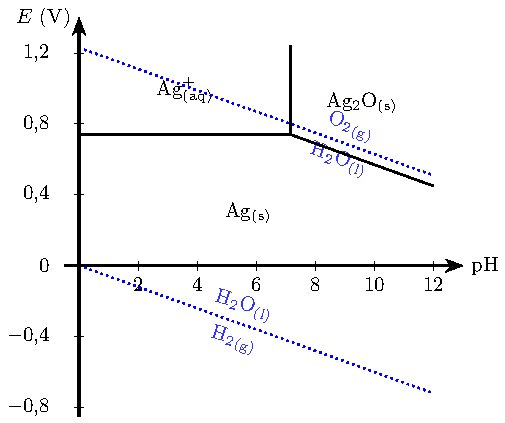
\includegraphics[width=\linewidth]{eph_ag-eau}
		\end{center}
	\end{minipage}
}%
\QR{%
	Établir l'équation de la frontière relative au couple $\ce{Ag^+/Ag}$.
}{%
	solu
}%
\QR{%
	Déterminer la pente de la frontière relative au couple $\ce{Ag_2O/Ag}$.
}{%
	solu
}%
\QR{%
	Qu'observe-t-on si on élève le pH d'une solution d'ions argent sans variation
	de la concentration initale en ions dans la solution~? Écrire l'équation de la
	réaction correspondante.
}{%
	solu
}%
\QR{%
	L'argent est-il stable dans l'eau~? Dans l'air~?
}{%
	solu
}%

\resetQ
\section{Diagramme $E-\pH$ du mercure}
\enonce{%
	\noindent
	\begin{minipage}[c]{.55\linewidth}
		L'allure du diagramme $E-\pH$ du mercure est donné ci-après. Les espèces prises
		en compte sont
		\[
			\ce{HgO_{\rm(s)}}
			\qquad
			\ce{{Hg}^2+_{\rm(aq)}}
			\qquad
			\ce{{Hg_2}^2+_{\rm(aq)}}
			\qquad
			\ce{Hg_{\rm(l)}}
		\]
		La concentration de chaque espèce dissoute comportant l'élément mercure aux
		frontières est prise égale à $c_0 = \SI{1.00}{mol.L^{-1}}$.
	\end{minipage}
	\hfill
	\begin{minipage}[c]{.40\linewidth}
		\vspace{0pt}
		\begin{center}
			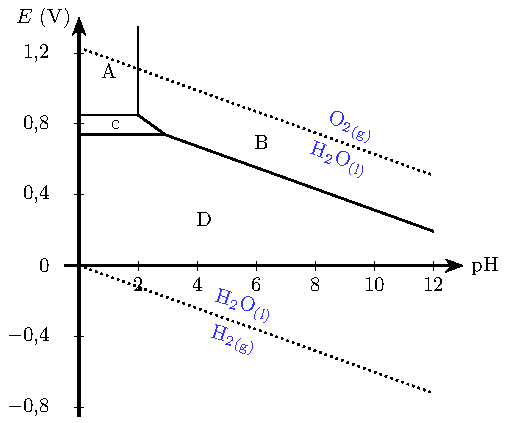
\includegraphics[width=\linewidth]{eph_hg-eau_plain}
		\end{center}
	\end{minipage}
}%

\QR{%
	Attribuer un domaine à chaque espèce, en précisant s'il s'agit d'un domaine de
	prédominance ou d'existence.
}{%
	solu
}%
\QR{%
	Le diagramme $E-\pH$ de l'eau a été tracé en pointillés. Le mercure métal
	est-il stable dans l'eau pure~? dans de l'eau «~aérée~» (c'est-à-dire avec de
	l'oxygène)~? Pour les situations instables, discutez de la nature des espèces
	créées en fonction des conditions du milieu.
}{%
	solu
}%
\QR{%
Retrouver la constante de l'équilibre $\ce{{Hg}^2+_{\rm(aq)} + 2
		{HO}^-_{\rm(aq)} = HgO_{\rm(s)} + H_2O_{\rm(l)}}$
}{%
solu
}%
\QR{%
	Calculer la pente de la frontière B/C.
}{%
	solu
}%
\QR{%
	Écrire l'équation bilan de la réaction ayant lieu lorsque l'on augmente le pH
	d'une solution aqueuse contenant l'espèce C. Comment appelle-t-on ce type de
	réaction~?
}{%
	solu
}%

\enonce{%
	Lorsque l'on veut tester la présence d'ions mercure en solution aqueuse, on
	peut opérer de la manière suivante~:
	«~\textit{Déposer une goutte de la solution aqueuse acidifiée à tester sur une
		lame de cuivre préalablement polie. Attendre quelques instants et laver la
		lame à l'eau. S'il se forme un amalgame blanc brillant sur la lame de cuivre, la
		solution contient des ions mercure}~».
	\smallbreak
	On indique qu'un amalgame est un alliage de mercure \ce{Hg} et d'un autre métal
	\ce{M}, noté \ce{MHg}. On donne $E^\circ (\ce{Cu^2+ /Cu}) = \SI{0.34}{V}$.
}%
\QR{%
	Pourquoi la solution à tester doit-elle être acidifiée~? Pour quels ions du
	mercure ce protocole est-il valable~? Écrire les équations bilans des
	réactions possibles en milieu acide.
}{%
	solu
}%

\resetQ
\section{Eau de Javel}
\enonce{%
	\noindent
	\begin{minipage}[c]{.55\linewidth}
		On dit souvent qu'il ne faut pas mélanger les produits ménagers, en
		particulier l'eau de Javel et un acide. Essayons de comprendre pourquoi.
		\smallbreak
		Le dichlore est un gaz toxique irritant, pouvant entraîner de graves problèmes
		pulmonaires en cas d'inhalation. Une solution aqueuse de dichlore
		$\ce{{Cl_2}_{\rm(aq)}}$ peut libérer du dichlore gazeux
		$\ce{{Cl_2}_{\rm(g)}}$. L'eau de Javel est une solution aqueuse comportant du
		chlorure de sodium $(\ce{{Na}^+_{\rm(aq)}};\ce{{Cl}^-}_{\rm(aq)})$ et de
		l'hypochlorite de sodium $(\ce{{Na}^+_{\rm(aq)}};\ce{{ClO}^-_{\rm(aq)}})$ en
		quantité équimolaire.
		\smallbreak
		Le diagramme potentiel-pH simplifié de l'élément chlore est représenté
		ci-contre, pour les espèces chimiques $\ce{HClO_{\rm(aq)}}$,
		$\ce{{ClO}^-_{\rm(aq)}}$, $\ce{{Cl_2}_{\rm(aq)}}$ et $\ce{{Cl}^-_{\rm(aq)}}$.
		La convention de tracé est fixée à $c_t = \SI{0.1}{mol.L^{-1}}$.
	\end{minipage}
	\hfill
	\begin{minipage}[c]{.45\linewidth}
		\vspace{0pt}
		\begin{center}
			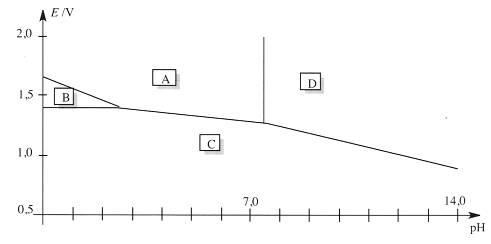
\includegraphics[width=\linewidth]{eph_javel-moche_white}
		\end{center}
	\end{minipage}
	\begin{tcb}(data)<lfnt>{Données}
		À \SI{298}{K} et $\pH = 0$, $E^\circ (\ce{HClO_{\rm(aq)}/{ClO_2}_{\rm(aq)}})
			= \SI{1.60}{V}$ et $E^\circ (\ce{{Cl_2}_{\rm(aq)}/{Cl}^-_{\rm(aq)}}) =
			\SI{1.39}{V}$.
	\end{tcb}
}%

\QR{%
	Indiquer les espèces chimiques auxquelles correspondent les domaines notés A,
	B, C et D.
}{%
	solu
}%
\QR{%
Retrouver graphiquement la valeur du $\pk$ du couple acido-basique
$\ce{HClO_{\rm(aq)}/{ClO}^-_{\rm(aq)}}$ et tracer le diagramme de prédominance
de ce couple. Quelle est l'espèce prédominante en milieu acide~?
}{%
solu
}%
\QR{%
	En utilisant le diagramme $E-\pH$, prévoir l'évolution d'un mélange contenant
	les espèces A et C lors du passage en milieu très acide $(\pH < \num{2.5})$.
	Écrire alors l'équation bilan de la réaction correspondante. Comment s'appelle
	une telle réaction~? Calculer sa constante d'équilibre à \SI{298}{K}.
}{%
	solu
}%
\QR{%
	Lorsque $\ce{{Cl_2}_{\rm(aq)}}$ se forme au sein de la solution, un équilibre
	s'établit alors avec $\ce{{Cl_2}_{\rm(g)}}$, ce qui entraîne un dégagement
	gazeux. Pourquoi ne faut-il donc jamais mélanger l'eau de Javel avec un
	acide~?
}{%
	solu
}%

\resetQ
\section{Autour du chrome}
\subsection{Diagramme $E-\pH$ du chrome}
\enonce{%
On donne le diagramme $E-\pH$ du chrome auquel se superpose celui de l'eau. On
étudie $\ce{{Cr}^2+_{\rm(aq)}}$, $\ce{{CrO_4}^2-_{\rm(aq)}}$,
$\ce{{CrO_2}^-_{\rm(aq)}}$, $\ce{{Cr}^3+_{\rm(aq)}}$,
$\ce{{Cr_2O_7}^2-_{\rm(aq)}}$, $\ce{Cr_{\rm(s)}}$ et
$\ce{{Cr(OH)_3}_{\rm(s)}}$. On donne $E^\circ (\ce{Cr^2+ /Cr}) =
	\SI{-0.91}{V}$.
}%
\QR{%
Dans cette question, on ne prend en compte que les espèces $\ce{{Cr}^2+_{\rm(aq)}}$,
$\ce{{CrO_2}^-_{\rm(aq)}}$, $\ce{{Cr}^3+_{\rm(aq)}}$, $\ce{Cr_{\rm(s)}}$ et
$\ce{{Cr(OH)_3}_{\rm(s)}}$. Indiquer pour chacun des domaines numérotés de 1 à 5
sur le diagramme à quelle espèce chimique il correspond, ainsi que la nature du
domaine.
}{%
solu
}%
\QR{%
	Déduire par lecture du diagramme la valeur de la concentration de tracé $c_t$,
	concentration de chaque espèce dissoute contenant l'élément chrome à la frontière.
}{%
	solu
}%
\QR{%
	Déduire du diagramme le $\pk[s]$ de $\ce{{Cr(OH)_3}_{\rm(s)}}$ ainsi que la
	constante de la réaction de dissolution de $\ce{{Cr(OH)_3}_{\rm(s)}}$ en
	milieu basique.
}{%
	solu
}%
\QR{%
On souhaite compléter le diagramme $E-\pH$ du chrome en prenant en compte, en
plus des espèces précédentes, les ions chromates $\ce{{CrO_4}^2-_{\rm(aq)}}$
et dichromates $\ce{{Cr_2O_7}^2-_{\rm(aq)}}$. Indiquer à quelle espèce
chimique correspond chacun des domaines numérotés 6 et 7.
}{%
solu
}%

\begin{center}
	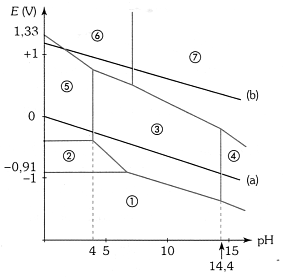
\includegraphics[width=.5\linewidth]{eph_cr-moche_white}
\end{center}

\subsection{Étude de réactions du chrome et de ses composés}
\begin{blocQR}
	\item \enonce{%
		Sur le diagramme précédent, on a également porté les droites délimitant le
		domaine de stabilité thermodynamique de l'eau.
	}%
	\QR{%
		Quels sont les composés du chrome au degré d'oxydation +\myRoman{6} qui sont
		stables en solution aqueuse~? Pour ceux qui seraient instables, on donnera
		l'équation de la réaction à laquelle ils donnent lieu.
	}{%
		solu
	}%
	\QR{%
	Les ions $\ce{{Cr}^3+_{\rm(aq)}}$ sont-ils stables en solution aqueuse~?
	Quelle(s) réaction(s) peuvent-ils donner avec l'eau~?
	}{%
	solu
	}%
	\item \enonce{%
		On étudie l'action du dichromate sur le fer II, en milieu de $\pH < 6$. Dans
		ces conditions, les potentiels des couples sont~:
		\begin{itemize}
			\item $\pH < \num{1.33}$~:
			      $E^\circ(\ce{{Fe}^3+_{\rm(aq)}/{Fe}^2+_{\rm(aq)}}) = \SI{0.77}{V}$~;
			\item $\num{1.33} < \pH < \num{6.5}$~: $E^\circ
				      (\ce{{Fe(OH)_3}_{\rm(s)}/{Fe}^3+}_{\rm(aq)}) = \num{1.01} - \num{0.18}\pH$
			      (en volts).
		\end{itemize}
		\QR{%
			Quels sont les produits obtenus par l'action du dichromate sur le fer II en
			milieu de $\pH < 6$~?
		}{%
			solu
		}%
		\begin{blocQR}
			\item \enonce{%
				On opère en général à pH voisin de 0.
			}%
			\QR{%
				Écrire l'équation de la réaction dans ce cas. Est-elle totale~?
			}{%
				solu
			}%
			\QR{%
				Commenter le choix du pH.
			}{%
				solu
			}%
			\QR{%
				L'utilisation du dichromate dans ces conditions est-elle en contradiction
				avec les résultats obtenus aux questions précédentes~?
			}{%
				solu
			}%
		\end{blocQR}
	}%
\end{blocQR}

\resetQ
\section{Dosage du glucose}
\enonce{%
	\noindent
	\begin{minipage}[c]{.55\linewidth}
		On donne l'allure du diagramme $E-\pH$ relatif aux substances iodées. On se
		limite aux espèces suivantes~: le diiode $\ce{{I_2}_{\rm(aq)}}$, les ions
		iodate $\ce{{IO_3}^-_{\rm(aq)}}$ et les ions iodure $\ce{{I}^-_{\rm(aq)}}$. La
		concentration de chacune des espèces iodées est égale à $c_t =
			\SI{0.10}{mol.L^{-1}}$ sur les frontières.
		\smallbreak
		On indique que le $\ce{{I_2}_{\rm(aq)}}$ a une coloration brune en solution,
		les autres espèces iodées sont incolores.
		\smallbreak
		On s'intéresser à un protocole permettant de déterminer la quantité de
		glucose dans une cannette de \textit{Redbull}. On détaille ci-dessous le
		protocole expérimental du dosage~:
	\end{minipage}
	\hfill
	\begin{minipage}[c]{.45\linewidth}
		\vspace{0pt}
		\begin{center}
			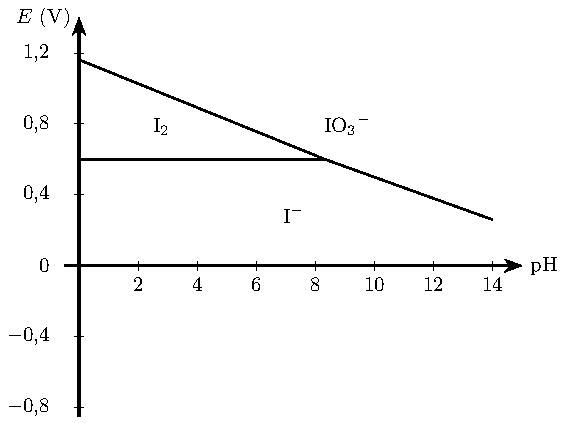
\includegraphics[width=\linewidth]{eph_iode}
		\end{center}
	\end{minipage}

	\begin{enumerate}[label=\clenumi]
		\item On introduit dans un erlenmeyer un volume $V_1 = \SI{20.0}{mL}$ d'une
		      solution de diiode de concentration $c_1 = \SI{0.050}{mol.L^{-1}}$~;
		\item On ajoute dans l'erlenmeyer $\SI{5}{mL}$ d'une solution d'hydroxyde de
		      sodium $(\ce{{Na}^+_{\rm(aq)}};\ce{{HO}^-_{\rm(aq)}})$ à
		      \SI{2.5}{mol.L^{-1}}. La solution se décolore.
		\item On ajoute au mélange précédent un volume $V_0 = \SI{2.0}{mL}$ de
		      \textit{Redbull}, de concentration en glucose $c_0$ inconnue. On
		      bouche l'erlenmeyer, on l'agite et on laisse agir 30 minutes dans
		      l'obscurité.
		\item Après cette attente, on ajoute dans l'erlenmeyer $\SI{10}{mL}$ d'acide
		      chlorhydrique $(\ce{{H}^+_{\rm(aq)}};\ce{{Cl}^-_{\rm(aq)}})$ à
		      \SI{2}{mol.L^{-1}}. La coloration brune réapparait.
		\item Une solution de thiosulfate de sodium
		      $(\ce{2{Na}^+_{\rm(aq)}};\ce{{S_2O_3}^2-_{\rm(aq)}})$ de concentration
		      $c_2 = \SI{0.10}{mol.L^{-1}}$ est introduite dans une burette. On
		      titre le contenu de l'erlenmeyer en présence d'empois d'amidon. On
		      observe alors une décoloration complète de la solution pour un volume
		      verse de thiosulfate de sodium noté $V\ind{2,eqv}$.
	\end{enumerate}
}%

\QR{%
	À la lumière du diagramme $E-\pH$ de l'iode, quelle réaction s'est produite
	lors de l'étape \circled{2}~? Écrire l'équation de cette réaction et nommer de
	type de réaction.
}{%
	solu
}%
\QR{%
Lors de l'étape \circled{3}, le glucose $\ce{{C_6H_12O_6}_{\rm(aq)}}$ est
oxydé en ions gluconates $\ce{{C_6H_11O_7}^-_{\rm(aq)}}$ par les ions iodates
en milieu basique. Écrire la réaction bilan qui se produit pendant cette
étape.
}{%
solu
}%
\QR{%
	À la lumière du diagramme $E-\pH$ de l'iode, quelle réaction s'est produite
	lors de l'étape \circled{4}~? Écrire l'équation de cette réaction et nommer de
	type de réaction.
}{%
	solu
}%
\QR{%
	Écrire l'équation de la réaction de titrage correspondant à l'étape
	\circled{5}. On indique que $E^\circ (\ce{{S_4O_6}^2-/{S_2O_3}^2-}) =
		\SI{0.09}{V}$ et $E^\circ (\ce{I_2/I^-}) = \SI{0.62}{V}$.
}{%
	solu
}%
\enonce{%
	Après avoir répété ce protocole trois fois, l'expérimentatrice mesure un
	volume moyen $V\ind{2,eqv} = \SI{15.4}{mL}$.
}%
\QR{%
	Exprimer littéralement, en fonction de $c_1$, $V_1$, $c_2$ et $V\ind{2,eqv}$
	la quantité d'ions iodates $n_3$ ayant réagi avec le glucose (étape
	\circled{3}). En supposant cette réaction totale, et en considérant que le
	glucose est le réactif limitant de cette réaction, en déduire la quantité de
	glucose $n_0$ ayant réagi. Calculer numériquement $c_0$.
}{%
	solu
}%
\QR{%
	Déduire de la question précédente la masse de glucose présente dans une
	canette de \textit{Redbull} de volume $V = \SI{250}{mL}$. La masse molaire du
	glucose est de $\SI{180}{g.mol^{-1}}$.
}{%
	solu
}%

\end{document}
